% Drawing 154/06-1 -- folder 154, batch 06, archive page 101 (PDF page 102).
% Transcription: page de dessins en couleur. À gauche, une carte en forme de disque : des faces pentagonales et hexagonales bordées de brun, des arcs orange et vert clair au bord, et le graphe dual tracé en bleu (sommets bleus au centre des faces, arêtes bleues qui traversent les arêtes brunes) ; des tirets en marge prolongent certaines arêtes. En haut à droite, au crayon, un cercle traversé de droites. Au milieu et en bas, deux droites horizontales vert clair coupées de droites orange, avec une courbe vert clair qui serpente autour d'elles (un balayage). Entre les deux, une rangée de petits triangles au crayon, certains hachurés, au-dessus et au-dessous d'une droite, avec de petites légendes au crayon, en partie lisibles : « \uncertain{pas de tr.} », « \uncertain{s-g}, $g$ », « \uncertain{pas de tr.} $s$-$g$ », et plus bas « \uncertain{à g.} ou à \uncertain{droite} » ; deux légendes à gauche sont biffées
% Kind: disk-shaped map with its dual; lines cut by pencils with a sweeping curve; pencil triangles. Method 2 (schematic redraw from the facsimile). Status: partial.
% Notes: Over a typed notice of the computing centre (not reproduced). Left: a disk-shaped map, pentagonal and hexagonal faces bordered in brown, orange and light green arcs at the rim, and the dual graph in blue (blue vertices at the centres of the faces, blue edges crossing the brown ones); dashes in the margin prolong some edges. Top right, in pencil, a circle crossed by lines. Middle and bottom: two light green horizontal lines cut by orange lines, with a light green curve winding round them (a sweep). Between them a row of small pencil triangles above and below a line, with small pencil legends (« pas de tr. », « s-g, g », « à g. ou à droite », partly read in the transcription; not reproduced). Read from the page view; the map is drawn as a central pentagon with a ring of faces, which is its structure on the page, but the outer faces are approximate and it is not encoded. Still differs from the facsimile: Over a typed notice of the computing centre (not reproduced). Between them a row of small pencil triangles above and below a line, with small pencil legends (« pas de tr. », « s-g, g », « à g. ou à droite », partly read in the transcription; not reproduced). Read from the page view; the map is drawn as a central pentagon with a ring of faces, which is its structure on the page, but the outer faces are approximate and it is not encoded. 6 coloured or hatched triangle(s) are placed schematically and are not bounded by the strands that bound them on the page.
% Coordinates: 1 unit = 1 mm = 1/100 of the crop width (bbox in page fractions: [0.202, 0.105, 0.9, 0.457]).
% Redrawn by Claude (claude-opus-5-5), issue #73, 2026-11-07; not checked by a human; not compiled (no TeX in the session).
% Revised by Claude (claude-opus-5-5) 2026-11-09 (issue #128) after Michel's check: vertices snapped to exact intersections (drawn points on their lines, meeting ends on the stroke they meet, near-concurrent lines through one computed point, curve ends on their rim); labels at \small as in folder 80 batch 3. Status: partial.
% Rights: reproduces part of the work -- behind RENDER_TRANSCRIPTS, never published by itself.
\documentclass[tikz,border=3pt]{standalone}
\usepackage{amsmath,amssymb}
\usetikzlibrary{patterns,arrows.meta}
\tikzset{Or/.style={orange!90!black}, Ye/.style={yellow!80!orange}, Lg/.style={green!60!black!70}, Dg/.style={green!45!black}, Br/.style={brown!80!black}, Rd/.style={red!85!black}, Bl/.style={blue!70!black}, Gy/.style={black!40}, pencil/.style={black!45}, struck/.style={black!35}, mark/.style={circle,draw,inner sep=1.3pt}, pt/.style={circle,fill,inner sep=0.9pt}, opt/.style={circle,draw,fill=white,inner sep=1.1pt}}
\begin{document}
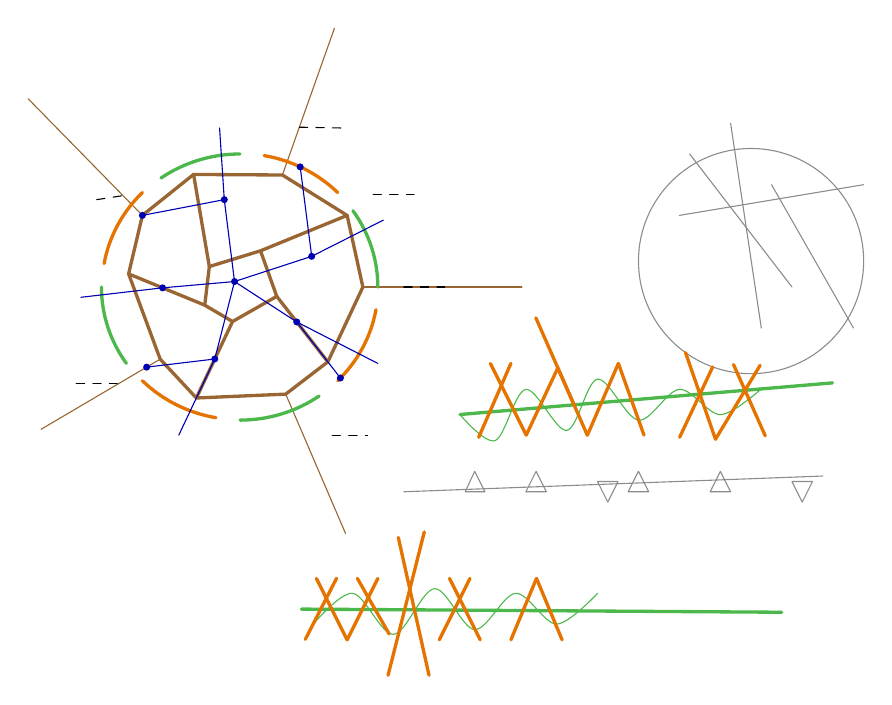
\begin{tikzpicture}[x=1mm,y=1mm,line cap=round,line join=round,font=\scriptsize]
\draw[Br,very thick] (16.9,-18.2) -- (23.4,-16.2) -- (25.46,-21.98) -- (19.85,-25.18) -- (16.32,-23.1) -- cycle;
\draw[Br,very thick] (16.9,-18.2) -- (14.9,-6.5);
\draw[Br,very thick] (23.4,-16.2) -- (34.4,-11.7);
\draw[Br,very thick] (25.46,-21.98) -- (31.95,-30.3);
\draw[Br,very thick] (19.85,-25.18) -- (15.25,-34.89);
\draw[Br,very thick] (16.32,-23.1) -- (6.65,-19.13);
\draw[Br,very thick] (14.9,-6.5) -- (26.18,-6.57) -- (34.4,-11.7) -- (36.4,-20.8) -- (31.95,-30.3) -- (26.6,-34.4) -- (15.25,-34.89) -- (10.66,-29.96) -- (6.65,-19.13) -- (8.4,-11.7) -- cycle;
\draw[Br] (26.18,-6.57) -- (32.79,12.07);
\draw[Br] (36.4,-20.8) -- (56.6,-20.8);
\draw[Br] (26.6,-34.4) -- (34.2,-52.1);
\draw[Br] (10.66,-29.96) -- (-4.48,-38.87);
\draw[Br] (8.4,-11.7) -- (-6.1,3.1);
\draw[Lg,very thick] (38.3,-20.8) arc[start angle=0, end angle=35, x radius=17.5, y radius=16.9];
\draw[Or,very thick] (33.2,-8.8) arc[start angle=45, end angle=80, x radius=17.5, y radius=16.9];
\draw[Lg,very thick] (20.8,-3.9) arc[start angle=90, end angle=125, x radius=17.5, y radius=16.9];
\draw[Or,very thick] (8.4,-8.8) arc[start angle=135, end angle=170, x radius=17.5, y radius=16.9];
\draw[Lg,very thick] (3.2,-20.8) arc[start angle=180, end angle=215, x radius=17.5, y radius=16.9];
\draw[Or,very thick] (8.4,-32.7) arc[start angle=225, end angle=260, x radius=17.5, y radius=16.9];
\draw[Lg,very thick] (20.8,-37.7) arc[start angle=270, end angle=305, x radius=17.5, y radius=16.9];
\draw[Or,very thick] (33.2,-32.7) arc[start angle=315, end angle=350, x radius=17.5, y radius=16.9];
\node[pt,Bl] at (20.1,-20.1) {};
\draw[Bl] (20.1,-20.1) -- (18.8,-9.7);
\draw[Bl] (20.1,-20.1) -- (29.9,-16.9);
\draw[Bl] (20.1,-20.1) -- (28,-25.23);
\draw[Bl] (20.1,-20.1) -- (17.59,-29.94);
\draw[Bl] (20.1,-20.1) -- (10.96,-20.9);
\node[pt,Bl] at (18.8,-9.7) {};
\node[pt,Bl] at (29.9,-16.9) {};
\node[pt,Bl] at (28,-25.23) {};
\node[pt,Bl] at (17.59,-29.94) {};
\node[pt,Bl] at (10.96,-20.9) {};
\node[pt,Bl] at (8.4,-11.7) {};
\node[pt,Bl] at (33.55,-32.35) {};
\node[pt,Bl] at (8.94,-30.97) {};
\node[pt,Bl] at (28.44,-5.54) {};
\draw[Bl] (18.8,-9.7) -- (18.2,-0.6);
\draw[Bl] (29.9,-16.9) -- (39,-12.3);
\draw[Bl] (28,-25.23) -- (38.3,-30.5);
\draw[Bl] (17.59,-29.94) -- (13.02,-39.61);
\draw[Bl] (10.96,-20.9) -- (0.6,-22.1);
\draw[Bl] (18.8,-9.7) -- (8.4,-11.7);
\draw[Bl] (29.9,-16.9) -- (28.44,-5.54);
\draw[Bl] (28,-25.23) -- (33.55,-32.35);
\draw[Bl] (17.59,-29.94) -- (8.94,-30.97);
\draw[dashed] (2.6,-9.7) -- (6.5,-9.1);
\draw[dashed] (0,-33.1) -- (5.2,-33.1);
\draw[dashed] (28.33,-0.5) -- (33.8,-0.6);
\draw[dashed] (37.7,-9.1) -- (42.9,-9.1);
\draw[dashed] (41.6,-20.8) -- (46.8,-20.8);
\draw[dashed] (32.5,-39.6) -- (37,-39.6);
\draw[pencil] (85.7,-17.5) circle[radius=14.3];
\draw[pencil] (77.9,-3.9) -- (90.9,-20.8);
\draw[pencil] (76.6,-11.7) -- (100,-7.8);
\draw[pencil] (83.1,0) -- (87,-26);
\draw[pencil] (88.3,-7.8) -- (98.7,-26);
\draw[Lg,very thick] (48.73,-36.99) -- (96.04,-32.97);
\draw[Lg] plot[smooth, tension=0.55] coordinates {(48.73,-36.99) (53.2,-40.3) (57.1,-33.8) (62.3,-39) (66.2,-32.5) (71.4,-37.7) (76.6,-33.8) (81.8,-37) (86.99,-33.74)};
\draw[Or,very thick] (51.11,-39.89) -- (55.2,-30.5);
\draw[Or,very thick] (57.15,-39.6) -- (61.16,-31.07);
\draw[Or,very thick] (64.91,-39.62) -- (68.85,-30.5);
\draw[Or,very thick] (76.63,-39.88) -- (80.83,-30.94);
\draw[Or,very thick] (81.18,-40.13) -- (86.85,-30.74);
\draw[Or,very thick] (57.15,-39.6) -- (52.6,-30.5);
\draw[Or,very thick] (64.91,-39.62) -- (61.16,-31.07);
\draw[Or,very thick] (72.1,-39.6) -- (68.85,-30.5);
\draw[Or,very thick] (81.18,-40.13) -- (77.38,-29.13);
\draw[Or,very thick] (87.5,-39.69) -- (83.47,-30.64);
\draw[Or,very thick] (58.37,-24.71) -- (63.22,-35.76);
\draw[pencil] (41.6,-46.8) -- (94.8,-44.8);
\draw[pencil] (49.4,-46.8) -- (50.6,-44.2) -- (51.9,-46.8) -- cycle;
\draw[pencil] (57.1,-46.8) -- (58.4,-44.2) -- (59.7,-46.8) -- cycle;
\draw[pencil] (70.1,-46.8) -- (71.4,-44.2) -- (72.7,-46.8) -- cycle;
\draw[pencil] (80.5,-46.8) -- (81.8,-44.2) -- (83.1,-46.8) -- cycle;
\draw[pencil] (66.2,-45.5) -- (67.5,-48.1) -- (68.8,-45.5) -- cycle;
\draw[pencil] (90.9,-45.5) -- (92.2,-48.1) -- (93.5,-45.5) -- cycle;
\draw[Lg,very thick] (28.6,-61.7) -- (89.6,-62.1);
\draw[Lg] plot[smooth, tension=0.55] coordinates {(30.05,-63.67) (35.1,-59.7) (40.3,-64.9) (45.5,-59.1) (50.6,-64.3) (55.8,-59.7) (61,-63.6) (66.2,-59.7)};
\draw[Or,very thick] (29.09,-65.54) -- (33.06,-57.78);
\draw[Or,very thick] (34.4,-65.6) -- (38.3,-57.8);
\draw[Or,very thick] (46.1,-65.6) -- (50,-57.8);
\draw[Or,very thick] (55.2,-65.6) -- (58.45,-57.8);
\draw[Or,very thick] (34.4,-65.6) -- (30.5,-57.8);
\draw[Or,very thick] (39.74,-64.86) -- (35.7,-57.8);
\draw[Or,very thick] (51.3,-65.6) -- (47.4,-57.8);
\draw[Or,very thick] (61.7,-65.6) -- (58.45,-57.8);
\draw[Or,very thick] (40.9,-52.6) -- (44.8,-70.1);
\draw[Or,very thick] (44.2,-51.9) -- (39.6,-70.1);
\end{tikzpicture}
\end{document}
